%
\chapter{Hilfsmittel/Arbeitsumgebung}
\label{chap:arbeit}

zum erstellen des Schaltplans und der Gerberfiles haben wir das auf den Laborrechnern bereitgestellte Tool Pulsonix verwendet.\\
Die Python Programmierung haben wir im Notepad++ durchgeführt.\\
Um den MSP430FR zu beschreiben griffen wir auf das vom Hersteller bereitgestellte Tool CCS zurück.

\subsection{Installation und anwendung des CCS}
\raggedright
Die aktuellste Version des CCS kann unter folgender URL bei ti direkt heruntergeladen werden \url{http://processors.wiki.ti.com/index.php/Download_CCS}.
Nach dem Ausführen der css\_setup.exe sollte im Schritt "processor support" wenigstens die Familie MSP430 wie in folgendem Screenshot gezeigt ausgewählt werden.\\
	\centering
	\fbox{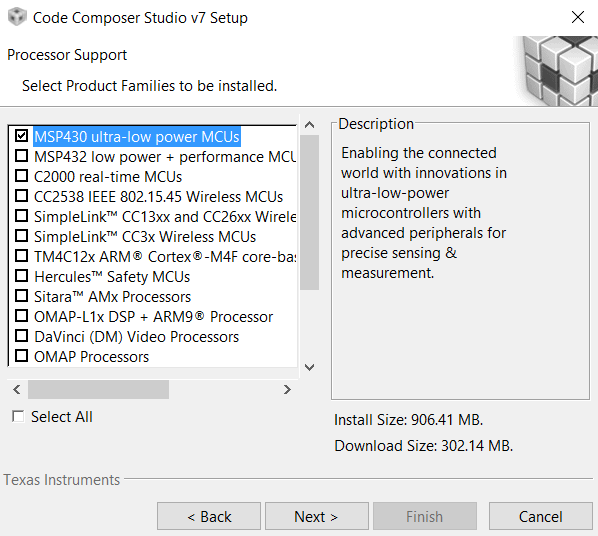
\includegraphics[width=0.5\textwidth]{media/ccs.png}}\\
\raggedright	
Nach der Installation des Programms kann ein Workspace angelegt oder ein bereits bestehender genutzt werden.
beim erstellen eines Neuen Projekts sollte darauf geachtet werden, dass auch der richtige Microcontroller ausgewählt wurde, folgender Screenshot zeigt die korrekte Einstellung\\
	\centering
	\fbox{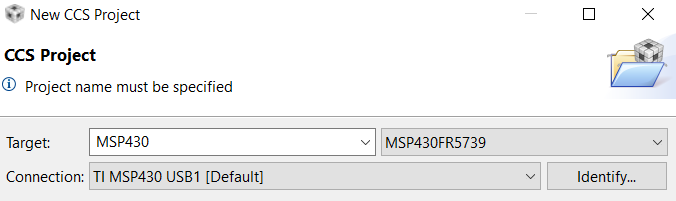
\includegraphics[width=0.5\textwidth]{media/ccs2.png}}\\
\raggedright	
durch diese Auswahl werden bereits die richtigen librarys eingebunden.
hier kann auch ein kleines Beispielprogramm erstellt werden, welches eine LED blinken lässt.
Die weitere Programmierung ist wie in herkömmlichen Entwicklungsumgebungen.
Eine nette und hilfreiche Erweiterung ist der Debugmodus, welcher uns schon oft weiter geholfen wird, hier kann das Programm auf dem MSP430 direkt laufengelassen, angehalten und fortgesetzt werden.



Ein bereits fertiger Workspace-Ordner mit allen hier aufgelisteten Programme ist auch auf der CD zu finden.